\def \serialnumtrials {1}
\def \serialblocksize {64}
\def \serialtable {
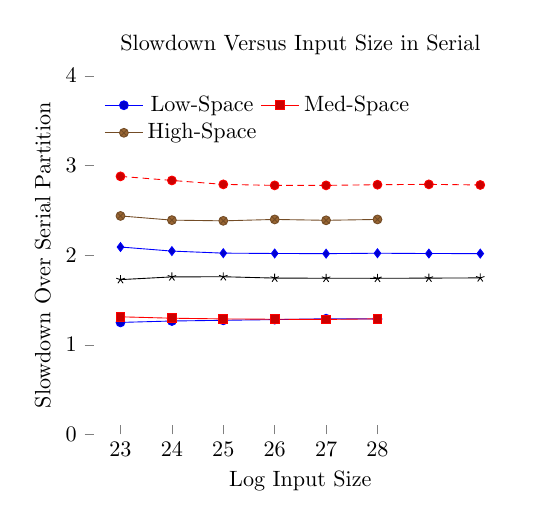
\begin{tikzpicture}[scale = .8]
\begin{axis}[
title={Slowdown Versus Input Size in Serial},
xtick pos=left,
ytick pos=left,
ymax = 4,
ymin = 0,
legend style={draw=none},
axis line style = { draw = none },
legend pos= north west,
xtick = data,
xlabel={Log Input Size},
ylabel={Slowdown Over Serial Partition},
legend columns = 2,
scatter/classes=%
{a={mark=o,draw=blue}}]
%% Serial Baseline
%% baselines in ms: \addplot coordinates {( 23, 32 ) ( 24, 64 ) ( 25, 128 ) ( 26, 256 ) ( 27, 512 ) ( 28, 1024 ) };
%% In-Place
\addplot coordinates {( 23, 1.25) ( 24, 1.26562) ( 25, 1.27344) ( 26, 1.28125) ( 27, 1.29102) ( 28, 1.28809) };
%% In-Place Prefix-Sum
\addplot coordinates {( 23, 1.3125) ( 24, 1.29688) ( 25, 1.28906) ( 26, 1.28516) ( 27, 1.2832) ( 28, 1.29004) };
%% Out-of-Place
\addplot coordinates {( 23, 2.4375) ( 24, 2.39062) ( 25, 2.38281) ( 26, 2.39844) ( 27, 2.38867) ( 28, 2.39844) };
\addplot coordinates {( 23, 1.72727) ( 24, 1.75758) ( 25, 1.7594) ( 26, 1.74436) ( 27, 1.74248) ( 28, 1.74178) ( 29, 1.74401) ( 30, 1.74654) };
%% In-Place Prefix-Sum
\addplot coordinates {( 23, 2.09091) ( 24, 2.04545) ( 25, 2.02256) ( 26, 2.0188) ( 27, 2.01692) ( 28, 2.0216) ( 29, 2.01832) ( 30, 2.01738) };
%% Out-of-Place
\addplot coordinates {( 23, 2.87879) ( 24, 2.83333) ( 25, 2.78947) ( 26, 2.7782) ( 27, 2.7782) ( 28, 2.78592) ( 29, 2.78957) ( 30, 2.78295) };

\legend{Low-Space, Med-Space, High-Space}
\end{axis}
\end{tikzpicture}
}
